\section{Introduction}
\subsection{Graph Partitioning}
Graph partitioning has been a standard problem in theoretical computer science for decades and has seen increasing attention as a method of partitioning problems to increase parallel locality. 


We wish to partition the nodes of a graph into $k$ balanced components with capacity $(1+\epsilon)\frac{N}{k}$, such that the number of edges that cross partition boundaries is minimized.
The number of inter-partition edges, which we seek to minimize, is often called the cost.
% While satisfying either the capacity constraint or the partitioning objective on their own is trivial, requiring both balanced and cost-minimization can be reduced to the minimum-bisection problem~\cite{Garey:1979:CIG:578533} and is therefore NP-Complete.
The process of balancing partition size while maintaining minimum cost can be reduced to the minimum-bisection problem~\cite{Garey:1979:CIG:578533} and is therefore NP-Complete.

\subsection{Why Use Streaming Partitioning?}
The most salient property of streaming partitioning is its speed: it can partition the graph in a single sweep, with $O(|E|)$ memory access, storage, and run time.
Existing graph partitioners require the whole graph to be represented in memory, whereas streaming graph partitioning can process vertices as they arrive.

As an example, partitioning a 26GB Twitter follower graph can take nearly a day using the fastest offline algorithms, but can take a matter of minutes using a streaming algorithm, with similar partition quality~\cite{tsourakakis2012fennel}.
This also suggests that we could do multiple passes of a streaming partitioner (using the same or different heuristics) to further improve the partitioning, all in a fraction of the time that an offline partitioner would take to terminate. 


\begin{figure}[h]
\centering
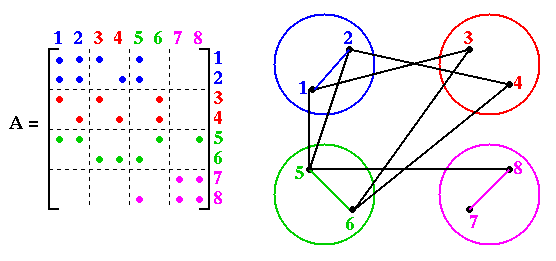
\includegraphics[width=0.8\columnwidth] {figures/graphpart.png}
\caption[Caption for]{Graph 4-partition shown with corresponding adjacency matrix \footnotemark}
\label{fig:0}
\end{figure}

% \footnotetext{Source: Jim Demmel's CS267 Lectures,~\url{http://www.cs.berkeley.edu/~demmel/cs267}}

Offline graph partitioning algorithms have existed for decades.
They work by allowing the graph to exist in memory with total information about the edges.
Hundreds of variants of these algorithms exist and range from spatial methods~\cite{Gilbert95geometricmesh} to spectral methods~\cite{arora2009expander}.
Some of the most scalable and effective graph partitioners are multi-level partitioners, which recursively contract the graph to a small number of vertices, and then heuristically optimize the problem on each subsequent expansion~\cite{karypis1998multilevel}. 

% Example
An effective partitioning of a graph can greatly improve the performance of graph algorithms.
Consider a parallel Breadth-First Search where a graph's vertices (vertex edge lists) are partitioned between two machines.
During each BFS step, each process must communicate all newly explored vertices to the owner of those vertices.
In Figure~\ref{fig:0}, if we have 4 processes, all 14 nonzeros in the non-diagonal blocks must be communicated at some point.
A good partitioner concentrates nonzeros in the diagonal blocks, thereby reducing communication (which is the main bottleneck in almost all graph computations). 

\section{Streaming Graph Partitioning}
Streaming graph partitioning has hained traction in the last few years~\cite{DBLP:journals/corr/abs-1212-1121,Stanton:2012:SGP:2339530.2339722,tsourakakis2012fennel}.
As graphs grow to the point where they do not fit into memory, or must be distributed to compute nodes on the fly we need methods that support partitioning on only limited information.
In the streaming model, input data (vertices) arrive sequentially from a generating source (such as a web-crawler), and must be partitioned as they arrive.

Streaming partitioning is dependent on the order in which vertices arrive.
A web crawler might generate vertices in an order that represents a Breadth-First or Depth-First traversal of the web, or we may receive vertices in a random order.
An analysis of streaming algorithms may also consider an adversarial ordering that produces the worst possible results~\cite{Stanton:2012:SGP:2339530.2339722}.
% We always consider a random ordering, because in the literature it is always on par with or better than other orderings. 
We have created \ourmethod, a fast, iterative, distributed streaming graph partitioner. 
\todo{somewhere need to mention the ordering. Maybe in eval?}
% We have investigated the effects of ordering on \ourmethod and find that random order often outperforms ordered traversals.


\subsection{Streaming Heuristics}
Given a stream of vertices, a heuristic makes a partition decision, given vertex $v$, and capacity constraint $C$ (where $C$ is generally $\approx \frac{(\epsilon+|V|)}{n}$ Stanton presents the following heuristics, roughly in order from most naive to most complex~\cite{Stanton:2012:SGP:2339530.2339722}: (only the un-buffered heuristics are presented)

\begin{enumerate}
\item \textbf{Balanced:} assign $v$ to partition of minimum size, with random tie breaking.
\item \textbf{Chunking:} divide input stream into chunks of size $C$.
\item \textbf{Hashing:} assign $v$ to $H(v)$, where $H$ is hash function $F:V\to\{1\dots k\}$
\item \textbf{Weighted Deterministic Greedy (WDG):} Assign $v$ to partition that it has most edges to, weighted by the relative size of each partition (weight function can be linear or exponential).
\item \textbf{Weighted Randomized Greedy:} Assign $v$ randomly according to a probability distribution defined by the weights of each partition in WDG.
\item \textbf{Weighted Triangles:} Assign $v$ to partition whose intersection with $v$ contains the most triangles, weighted by the relative size of each partition.
\item \textbf{Balance Big:} for high-degree $v$, use Balanced. For low-degree $v$, use WDG. 
\end{enumerate}

Of note is that many major graph-processing toolkits such as GraphLab~\cite{Low:2012:DGF:2212351.2212354} use the hashed (random) partitioning method, which essentially produces a worst-case edgecut of size $\frac{k-1}{k}|E|$, but which has the benefit that $H(v)$ can be called at any time to return the compute node that owns $v$.


In Stanton's experimental results~\cite{Stanton:2012:SGP:2339530.2339722}, WDG performed far better than any other partitioner.
FENNEL~\cite{tsourakakis2012fennel} is a heuristic that generalizes the WDG partitioner for any weight function, and provides a somewhat more rigorous theoretical framework.
For this project, we always consider a WDG partitioner. 

